\documentclass[xcolor=dvipsnames]{beamer}




\usepackage{BOO}
\usepackage{natbib}
\usepackage{linguex}
\usetheme{Boadilla}

\usepackage{amssymb,amsmath,stmaryrd,qtree,graphicx}
\usepackage{soul}
\usepackage{rotating}

\usepackage{tikz,pgf}
\usetikzlibrary{arrows,fit}
\usepackage{pgfplots}

\newcommand{\be}{\begin{enumerate}}
\newcommand{\ee}{\end{enumerate}}
\newcommand{\bi}{\begin{itemize}}
\newcommand{\ei}{\end{itemize}}

\newcommand{\ought}{\ensuremath{{O}}}
\newcommand{\may}{\ensuremath{{M}}}
\newcommand{\p}{\ensuremath{\blacklozenge}}
\newcommand{\term}[1]{\textbf{\emph{#1}}}
\newcommand{\dor}{\mathrel{\text{\sc{or}}}}
\newcommand{\May}{\mathop{\text{\sc{may}}}}
\newcommand{\Ought}{\mathop{\text{\sc{ought}}}}

\title{Deontic Disjunction}
\author[Melissa Fusco]{Melissa Fusco \\ Meaning Sciences Club}
\date{September 30, 2014}

\begin{document}

%--- the titlepage frame -------------------------%
\begin{frame}[plain]
  \titlepage
\end{frame}

\begin{frame}
\begin{center}
{\LARGE \textcolor{RoyalBlue}{Two Puzzles}}
\end{center}
\end{frame}


\begin{frame}{Free Choice Permission}
\begin{center}
\ex. You may have the gin or the whiskey.\\
$\May (G \dor W)$ \label{gin} \\ 

\vspace{30pt}
\pause

 \textcolor{RoyalBlue}{(FC)} $\quad \May(\phi \dor \psi) \Rightarrow \May \phi \wedge \May \psi$. \\ 
 \vspace{10pt}
 \pause
  \textcolor{RoyalBlue}{(Exclusivity)} $\quad \May(\phi \dor \psi) \nRightarrow \May (\phi \wedge \psi)$. 
    \end{center}
    \end{frame}

\begin{frame}{Ross's Puzzle}
\begin{center}
  \ex. I ought to post the letter. \\
$\Ought (R)$ \label{post} \\ 

\pause

\ex. I ought to post the letter or burn it. \\
$\Ought (R \dor B)$ \label{burn} \\ 


\vspace{30pt}
\pause

 \textcolor{RoyalBlue}{(R)} $\quad \Ought(\phi) \nRightarrow \Ought(\psi \dor \psi)$. \\ 
 \vspace{10pt}
 
 \pause
 
  \textcolor{RoyalBlue}{(R+)} $\quad \Ought(\phi \dor \psi) \Rightarrow \May \phi \wedge \May \psi)$. 
    \end{center}
    \end{frame}

    
%%%%%%
    
\begin{frame}{Sayre-McCord's Observation}
  
\begin{center}
$\Ought(\phi) \nRightarrow \Ought(\phi \dor \psi)$
\end{center}
\vspace{10pt}
%Boo! \BOO
%
\cite{Enderton:1972}
\pause
\ex. Ralph may go to the movies.

\pause

\ex. Ralph ought to pay back his loan. 

\pause

\ex. Ralph ought to pay back his loan or go to the movies.

\pause

\vspace{10pt}
\begin{center}
  \textcolor{RoyalBlue}{(SM)} $\May(\psi) \wedge \Ought(\phi) \nRightarrow \Ought(\phi \dor \psi)$
\end{center}

\end{frame}

\begin{frame}{Sayre-McCord's Observation}
\begin{center}
  \textcolor{RoyalBlue}{(Conditionals-1)}\\ I may do ($\phi \dor \psi$) $\Rightarrow$ If I do not do $\phi$, I may do $\psi$; \\ 
  
  I may do ($\phi \dor \psi$) $\Rightarrow$ If I do not do $\psi$, I may do $\phi$. 
  \pause
  \vspace{30 pt}
 
 \textcolor{RoyalBlue}{(Conditionals-2)}\\ I ought to do ($\phi \dor \psi$) $\Rightarrow$ If I do not do $\phi$, I ought to do $\psi$; \\ 
  
  I ought to do ($\phi \dor \psi$) $\Rightarrow$ If I do not do $\psi$, I ought to do $\phi$. 
  
\end{center}
\end{frame}

\begin{frame}
\begin{table}[H]
\centering

\begin{tabular}{ll}
\textbf{May:} & \\
(Failure of `or' intro) & $\May \phi \nRightarrow \May(\phi \dor \psi)$ \\
(FC) & $\May(\phi \dor \psi) \Rightarrow \May \phi, \May \psi$ \\
(Conditionals 2) & $\May(\phi \dor \psi) \Rightarrow \text{if } \neg \phi \text{, then } \May \psi$ \\
\\
\textbf{Ought:} & \\
(Failure of `or' intro) & $\Ought \phi \nRightarrow \Ought(\phi \dor \psi)$ \\
(R+) & $\Ought(\phi \dor \psi) \Rightarrow \May \phi, \May \psi$ \\
(Conditionals 1) & $\Ought(\phi \dor \psi) \Rightarrow \text{if } \neg \phi \text{, then } \Ought \psi$
\end{tabular}

\caption {Data for `ought' and `may'.} 
\label{tab:data}
\end{table}

\end{frame}

\begin{frame}
\begin{center}
{\LARGE \textcolor{RoyalBlue}{Proto-Semantics with Kripke Frames}\\$~$\\}
%
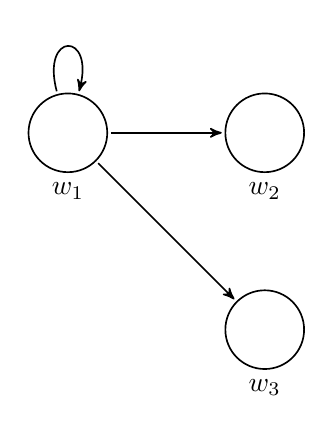
\begin{tikzpicture}[->,>=stealth',shorten >=1pt,shorten <=1pt, auto,node
distance=2.5cm,semithick]
\tikzstyle{every state}=[fill=gray!20,draw=none,text=black]
\node[circle,draw=black,label=below:$w_1$,minimum size=1cm] (w1)  {$~$};
\node[circle,draw=black,label=below:$w_2$,minimum size=1cm] (w2) [right of=w1] {$~$};
\node[circle,draw=black,label=below:$w_3$,minimum size=1cm] (w3) [below of=w2] {$~$};
%\path (w2) edge[loop right] node { } (w2);
\path (w1) edge[loop above] node {} (w2);
\path (w1) edge[->] node {} (w2);
\path (w1) edge[->] node {} (w3);


%\node[draw, thick, rounded corners, inner sep=2em, fit=(w1) (w2)] {};
\end{tikzpicture}
%
%\caption{$s_\textrm{nice} = \{w_1, w_2\}$}
%\label{fig:nice}
%\end{figure}

\end{center}
\end{frame}

\begin{frame}{Proto-Semantics with Kripke Frames}
\begin{definition}[Circumstantial Possibility]
$\phi$ is \term{circumstantially possible at $s$} iff $\exists w' \in s$ such that $\phi$ is true at $w'$.
\end{definition}

%\begin{dfn}[Acceptance]
%$\phi$ is \term{accepted at $s$} iff $\forall w' \in s$, $\phi$ is true at $w'$.
%\end{dfn}

\end{frame}

%%%%%%%%%%%%%%%%%%%%%%%%%%%%%%%%%%%%%

\begin{frame}
\begin{center}
{\LARGE \textcolor{RoyalBlue}{Thank You!}}
\end{center}
\end{frame}

\begin{frame}{Bibliography}
\bibliographystyle{philosophy}
\bibliography{Dreamboat}

\end{frame}
\end{document}